\documentclass[a4paper,UTF8]{ctexart}

\usepackage{amsmath, amsthm, amssymb, amsfonts, hyperref, mathrsfs}%美国数学学会的包+?
\usepackage{geometry} %控制界面
\usepackage{bookmark}
\usepackage{fancyhdr} % header & footer
\usepackage{appendix} % 附录
\usepackage{tikz} %作图
\usepackage{graphicx} %插入图片的宏包
\usepackage{float} %设置图片浮动位置的宏包
\usepackage{subfigure} %插入多图时用子图显示的宏包
\usepackage{listings} %引用代码
\usepackage{physics,mathtools} %物理数学工具
\usepackage{comment}
\usepackage{framed}
\geometry{top=2.5cm,bottom=2.5cm,left=2.5cm,right=2.5cm} % 布局要求
\pagestyle{fancy} % fancy分格
\fancyhf{} % 清除所有页眉页脚
\renewcommand\headrulewidth{0.6pt}
\renewcommand\footrulewidth{0.6pt}
\lhead{何金铭 PB21020660$\mid$座位号:3}
\chead{$\beta$吸收2实验报告}
\rhead{\thepage}
\lfoot{2023.4.3}
\rfoot{USTC}
%\bibliographystyle{plain} % 引用样式
\everymath{\displaystyle} % display
%============================================================

\begin{document}

\begin{center}
    \textbf{\Large $\beta$吸收2实验报告}
    \par \text{\large 何金铭 PB21020660}
\end{center}

\section{实验目的}

\begin{enumerate}
    \item 学习产生单能电子束的原理
    \item 学习$\beta$磁谱仪的原理与使用
    \item 学习闪烁能谱仪的使用
    \item 验证高速电子的动量与动能关系
    \item 测量吸收片对单能电子束的吸收曲线
\end{enumerate}

\section{实验原理}

\subsection{电子动量的测量}

本实验采用半圆聚焦$\beta$磁谱仪测量电子的动量,若轨道半径为R,则与电子动量p有关系式:

\begin{equation}
    p = eBR
\end{equation}

\begin{figure}[H]
    \centering
    \begin{minipage}[b]{0.9\textwidth}
        \centering
        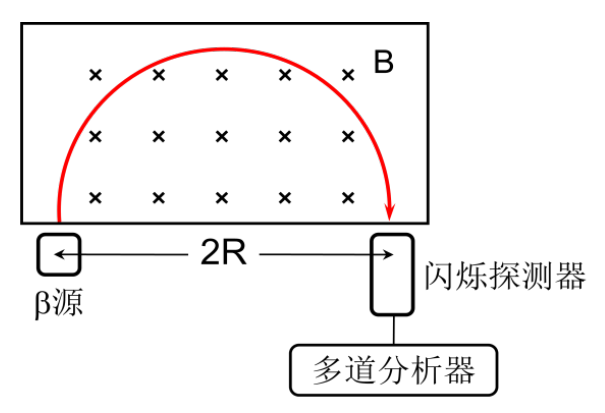
\includegraphics[width=0.4\textwidth]{./m.png}
        \caption{半圆聚焦$\beta$磁谱仪与闪烁能谱仪示意图}
    \end{minipage}
\end{figure}

\subsection{电子动能的测量}

利用$^{137}Cs$的$\gamma$射线能谱对闪烁能谱仪进行定标。动能的大小与能谱的峰位N成线性关系:

\begin{equation}
    E = aN + b
\end{equation}

式中a,b为待定系数。

\subsection{相对论效应}

相对性粒子有动能$E_k$与动量$p$的关系:

\begin{equation}
    E_{k} = \sqrt{p^2c^2 + m_{0}^{2}c^4}-m_{0}c^2
\end{equation}

其中,为计算方便,实验室中的动量可用$pc$表示:

且有:

\begin{equation}
    pc = eBRc(J) = 300BR (MeV)
\end{equation}

\subsection{单能电子束的获得}

由于发生衰变的原子核在发射$\beta$粒子的同时还放出中微子,两者分配能量的
结果导致发射出的$\beta$粒子能谱为 0 至最大动能$E_{max}$之间连续分布的能谱,在磁谱
仪中的偏转半径也各不相同,具有相同动能的$\beta$粒子在$\beta$磁谱仪中的偏转半径也相
同。据此,我们可以在闪烁探头前开一条与磁场平行的狭缝,只让某一偏转半径
的$\beta$粒子进入闪烁探测器。只要狭缝足够窄,就可以认为进入闪烁探测器的就是
单能电子束,闪烁能谱仪测出的就是该单能电子束的能谱。

\subsection{测量物质对电能电子束的吸收曲线}

考虑一束初始强度为$I_0$的单能电子束,当穿过厚度为 x 的物质时,强度减
弱为 I。强度 I 随厚度 x 的增加而减小且服从指数规律,可表示为:

\begin{equation}
    I = I_0 e^{-\mu x}
\end{equation}

式中$\mu$为该物质的线性吸收系数。可以做变换:设质量吸收系数$\mu_{m}=\mu / \rho$,质量厚度为$d = \rho x$,有

\begin{equation}
    I = I_0 e^{-\mu_{m}d}
\end{equation}

\section{实验仪器}

闪烁$\gamma$能谱仪,半圆聚焦$\beta$磁谱仪,吸收片,$^{137}Cs$放射源,$^{90}Sr-^{90}\gamma$放射源,电子秤,狭缝,直尺

\section{原始实验数据}

\subsection{3号台的一些基本数据}

\begin{enumerate}
    \item 磁谱仪中产生的磁感应强度为B = 622.78 Gs
    \item 电子入射闪烁体前铝制入射窗产生的能量损失为$\Delta E$ = 0.09MeV
    \item 实验室的铝片质量厚度为$d = 50mg/cm^2$
\end{enumerate}

\subsection{闪烁能谱仪定标}

\begin{table}[H]
    \centering
    \begin{tabular}{|c|c|c|}
    \hline
        E/MeV & 0.184MeV & 0.662MeV \\ \hline
        峰位N & 89 & 287.14 \\ \hline
    \end{tabular}
    \caption{$^{137}Cs$的$\gamma$能谱部分数据记录表}
\end{table}

{\bfseries 注:}3号台的实验仪器存在一些问题,$E = 0.184MeV$处峰位值无精确读数,$N=89$为大致读数

\subsection{$\beta$射线能谱}

\begin{table}[H]
    \centering
    \begin{tabular}{|c|c|c|c|c|c|c|c|c|}
    \hline
        ~ & 1 & 2 & 3 & 4 & 5 & 6 & 7 & 8 \\ \hline
        x/cm & 23 & 24.5 & 26.0 & 27.5 & 29.0 & 30.5 & 32 & 33.5 \\ \hline
        峰位N & 219.78 & 281.33 & 336.29 & 392.47 & 444.78 & 493.73 & 529.98 & 579.39 \\ \hline
    \end{tabular}
    \caption{$\beta$能谱数据记录表}
\end{table}

\subsection{$\beta$吸收数据}

\begin{table}[H]
    \centering
    \begin{tabular}{|c|c|c|c|c|}
    \hline
        铝片数量 & 峰位 & FWHM & 选区计数 & 采集时间/s \\ \hline
        0 & 407.31 & 100.23 & 72613 & 200 \\ \hline
        1 & 374.46 & 87.46 & 51713 & 200 \\ \hline
        2 & 344.34 & 75.53 & 37055 & 200 \\ \hline
        3 & 313.78 & 121.77 & 54226 & 300 \\ \hline
        4 & 269.27 & 112.99 & 61889 & 400 \\ \hline
    \end{tabular}
    \caption{$x=28cm$时铝片吸收数据记录表}
\end{table}

\section{数据处理}

\subsection{闪烁能谱仪的定标}

将$E_1 = 0.184 MeV,N_1 = 89$和$E_2 = 0.662MeV,N_2 = 287.14$代入$E= aN +b$得:
$a = 2.412 \times 10^{-3} MeV,b = -3.071 \times 10^{-2} MeV$。

将$a,b,\Delta E$代入$E = aN+b + \Delta E$,可以得到标定的能量公式为:

\begin{equation}
    E = 0.0024 N + 0.0593 (MeV)
\end{equation}

\subsection{$\beta$射线能谱}

利用公式:

\begin{equation}
    R = \frac{x-10cm}{2}
\end{equation}

\begin{equation}
    pc = 300BR (MeV)
\end{equation}

\begin{equation}
    E_{classic} = \frac{(pc)^2}{2mc^2}
\end{equation}

\begin{equation}
    E_{relative} = \sqrt{p^2c^2 + m^{2}c^4}-mc^2
\end{equation}

\begin{equation}
    E_{measure} = 0.0024 N + 0.0593 (MeV)
\end{equation}

可以计算得以下结果:

\begin{table}[H]
    \centering
    \begin{tabular}{|c|c|c|c|c|c|c|c|c|}
    \hline
        ~ & 1 & 2 & 3 & 4 & 5 & 6 & 7 & 8 \\ \hline
        x/cm & 23 & 24.5 & 26.0 & 27.5 & 29.0 & 30.5 & 32 & 33.5 \\ \hline
        R/cm & 6.5 & 7.25 & 8 & 8.75 & 9.5 & 10.25 & 11 & 11.75 \\ \hline
        pc/MeV & 1.214 & 1.355 & 1.495 & 1.635 & 1.775 & 1.915 & 2.055 & 2.195 \\ \hline
        峰位N & 219.78 & 281.33 & 336.29 & 392.47 & 444.78 & 493.73 & 529.98 & 579.39 \\ \hline
        经典动能$E_{classic}$/MeV & 1.442 & 1.797 & 2.187 & 2.616 & 3.083 & 3.588 & 4.132 & 4.714 \\ \hline
        相对论动能$E_{relative}$/MeV & 0.806 & 0.937 & 1.069 & 1.202 & 1.336 & 1.471 & 1.607 & 1.743 \\ \hline
        $E_{measure}$/MeV & 0.587 & 0.734 & 0.866 & 1.001 & 1.127 & 1.244 & 1.331 & 1.450 \\ \hline
        $\left\lvert E_{measure}-E_{relative}\right\rvert $ & 0.219 & 0.203 & 0.203 &0.201 & 0.209 &0.227 & 0.276 & 0.293 \\ \hline    \end{tabular}
    \caption{$\beta$能谱分析数据表}
\end{table}

\begin{figure}[H]
    \centering
    \begin{minipage}[b]{0.9\textwidth}
        \centering
        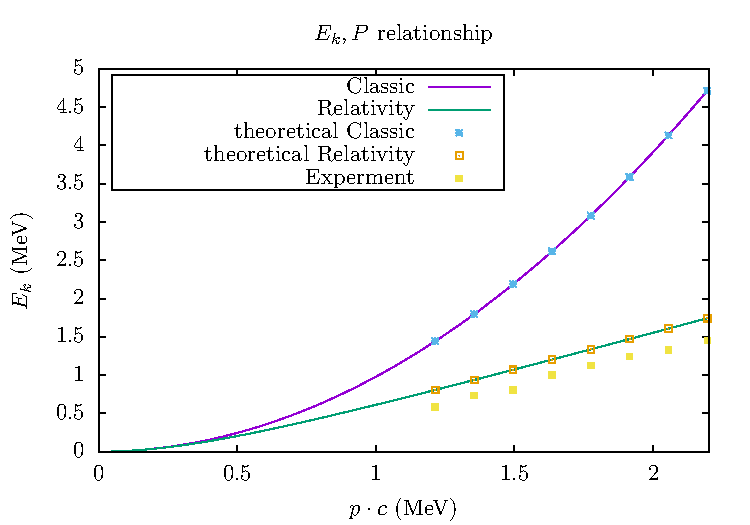
\includegraphics[width=0.9\textwidth]{./pic.pdf}
        \caption{经典力学、相对论力学与实验测量的$E_{k}$,pc值对比图}
    \end{minipage}
\end{figure}

可以发现:

\begin{enumerate}
    \item 在高速情况下,经典力学的理论动能会大于相对论力学的理论动能
    \item 实验测得的动能均小于相对论力学的理论动能,但是于不同的位置下,减少的动能几乎一致(可见上表中最后一行),可能是由于某一系统误差导致的。
\end{enumerate}

\subsection{$\beta$吸收实验}

于实验中,我们设置$\beta$射线在磁谱仪中运动的半径为$R= \frac{28cm-10cm}{2} = 9 cm$,可以计算
得$pc = 300 B R = 1.682 MeV$,从而进一步可以计算得其动能为:

\begin{equation}
    E_{k} = \sqrt{(pc)^2+m^2c^4}-mc^2 = 1.247 MeV
\end{equation}

\begin{table}[H]
    \centering
    \begin{tabular}{|c|c|c|c|c|c|}
    \hline
        铝片数量 & 峰位 & FWHM & 选区计数 & 采集时间/s & 单位时间入射粒子数I/s \\ \hline
        0 & 407.31 & 100.23 & 72613 & 200 & 363.07 \\ \hline
        1 & 374.46 & 87.46 & 51713 & 200 & 258.565 \\ \hline
        2 & 344.34 & 75.53 & 37055 & 200 & 185.275 \\ \hline
        3 & 313.78 & 121.77 & 54226 & 300 & 180.753 \\ \hline
        4 & 269.27 & 112.99 & 61889 & 400 & 154.723 \\ \hline
    \end{tabular}
    \caption{$\beta$吸收数据处理表1}
\end{table}

下面验证吸收公式$I = I_{0} e^{-\mu_{m}d}$是否正确,变换为:

\begin{equation}
    \ln{\frac{I}{I_0}} = -\mu_{m} d 
\end{equation}

其中$d_0$为单位铝片的厚度,d为铝片的质量厚度,处理实验数据得下表:

\begin{table}[H]
    \centering
    \begin{tabular}{|c|c|c|c|c|}
    \hline
        d/($50mg/cm^2$) & 1 & 2 & 3 & 4 \\ \hline
        $\ln{\frac{I}{I_0}}$ & -0.339 & -0.673 & -0.697 & -0.853 \\ \hline
    \end{tabular}
    \caption{$\beta$吸收数据处理表2}
\end{table}

\begin{figure}[H]
    \centering
    \begin{minipage}[b]{0.9\textwidth}
        \centering
        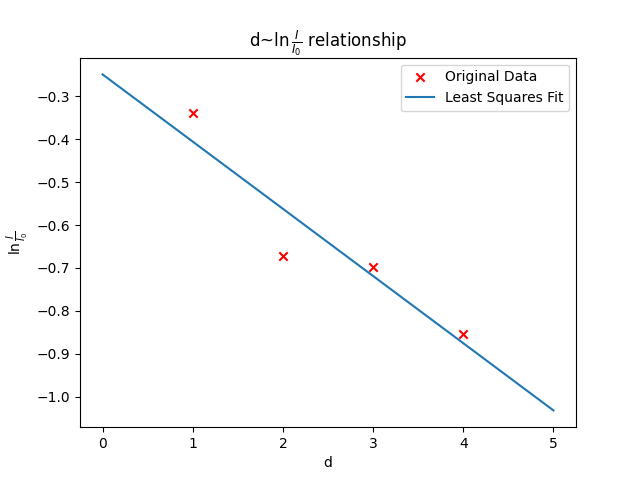
\includegraphics[width=0.8\textwidth]{./fit.png}
        \caption{$d$-$\ln{\frac{I}{I_0}}$拟合曲线}
    \end{minipage}
\end{figure}

拟合得:

\begin{equation}
    \ln{\frac{I}{I_0}} = -0.157 d - 0.249
\end{equation}

取其斜率$\mu_m = -0.157 (0.02cm^2/mg) = -0.00314 cm^2/mg$

所以估计得:$I = I_0 e^{-0.00314d}$其中d的单位为$mg/cm^2$

\section{实验总结和误差分析}

\subsection{误差分析}

\subsubsection{$\beta$磁谱仪实验结果的误差分析}

实验测得的$\beta$射线的动能与相对论预言的结果类似,但是有一些偏差:对于不同动量的$\beta$射线,实验值比理论值少了
约0.229MeV的能量,可能的原因有:

\begin{enumerate}
    \item 整个实验有一个系统误差,比如:闪烁体的修正$\Delta E$的修正值不正确;空气以及一些其它的因素对$\beta$射线也有衰减作用。
    \item 仅仅利用$\gamma$能谱的两个点来对闪烁能谱仪进行定标存在极大的误差,对截距$b$的影响很大,从而引起了一个比较大的整体误差,需要利用更多的特征点或者其它的能谱来对其进行定标。
\end{enumerate}

\subsubsection{$\beta$吸收的实验结果的误差分析}

实验测得峰位和FWHM(半高宽)的关系不太正常,按理论,随着铝片数量的增加,峰位应该减小,而FWHM应该增大;但是实验观察到的现象为FWHM先减小,后增大。

可能的原因是

\begin{enumerate}
    \item 在测量FWHM时,选择不同的选区结果可能会有不同,由于没有规定一个统一的选区标准,导致FWHM不同,这里需要指出:
    将选区选的过大不会有什么影响,但是选区过小则会导致FWHM过小,上述的结果就可能是由于这个原因导致的。
    \item 可能由于狭缝存在一点宽度,无铝片的时候导致FWHM过宽,而由于铝片的衰减作用,会筛选出最多的$\beta$射线或能量最大的$\beta$射线
    使得1,2片的铝片FWHM变小;而加3片以上时,衰减作用过强,导致FWHM又变大。
\end{enumerate}

之后拟合的曲线的误差也源于此处。

\subsection{实验总结}

\begin{enumerate}
    \item 了解了单能电子束的原理,学习了$\beta$磁谱仪、闪烁能谱仪的原理和使用
    \item 对闪烁能谱仪进行了定标,得到的转换公式为$E = 0.0024N + 0.0593(MeV)$
    \item 检验了高速电子的动量与动能的关系,发现高速电子的动量与能量的关系更符合于相对论力学,但存在一些系统误差,认为可能是由于
    装置对电子的损失能量$\Delta E$少计算了一部分。
    \item 计算得铝片对$\beta$射线的吸收曲线近似为$I = I_0 e^{-0.00314d}$其中d为质量厚度,其单位为$mg/cm^2$
\end{enumerate}

\end{document}